%------------------------------------------------------------------------------
%   PACKAGES AND OTHER DOCUMENT CONFIGURATIONS
%------------------------------------------------------------------------------

\documentclass[twoside,twocolumn]{article}

\usepackage[english]{babel} % Language hyphenation and typographical rules

% Document margins
\usepackage[hmarginratio=1:1,top=32mm,left=20mm,right=20mm,columnsep=20pt]{geometry}
% Custom captions under/above floats in tables or figures
\usepackage[hang, small,labelfont=bf,up,textfont=it,up]{caption}
\usepackage{booktabs} % Horizontal rules in tables

\usepackage{enumitem} % Customized lists
\setlist[itemize]{noitemsep} % Make itemize lists more compact
\usepackage{textcomp}

% Allows abstract customization
\usepackage{abstract}
% Set the "Abstract" text to bold
\renewcommand{\abstractnamefont}{\normalfont\bfseries}
% Set the abstract itself to small italic text
\renewcommand{\abstracttextfont}{\normalfont\small\itshape}

\usepackage{fancyhdr} % Headers and footers
\pagestyle{fancy} % All pages have headers and footers
\fancyhead{} % Blank out the default header
\fancyfoot{} % Blank out the default footer
\fancyhead[C]{\thetitle}
\fancyfoot[RO,LE]{\thepage} % Custom footer text

\usepackage{titling} % Customizing the title section

\usepackage{hyperref} % For hyperlinks in the PDF
\usepackage{amsmath}

\usepackage{tikz}
\usetikzlibrary{bayesnet}
\usetikzlibrary{arrows}

\usepackage{color}
\usepackage{caption}
\usepackage{subcaption}

\usepackage{graphicx}

\captionsetup[figure]{labelfont={bf},textfont=normalfont}

%------------------------------------------------------------------------------
%   TITLE SECTION
%------------------------------------------------------------------------------

\setlength{\droptitle}{-4\baselineskip} % Move the title up

\pretitle{\begin{center}\Huge\bfseries} % Article title formatting
\posttitle{\end{center}} % Article title closing formatting

\title{Machine Translation Project Proposal: \\ Using Neural Networks to Learn
Word Alignments}
\author{%
\textsc{Bailey Parker} \\[1ex]
\normalsize Johns Hopkins University \\
\normalsize \href{mailto:bailey@jhu.edu}{bailey@jhu.edu}
 \and
 \textsc{Vivian Tsai} \\[1ex]
\normalsize Johns Hopkins University \\
\normalsize \href{mailto:viv@jhu.edu}{viv@jhu.edu}
 \and
  \textsc{William Watson} \\[1ex]
\normalsize Johns Hopkins University \\
\normalsize \href{mailto:wwatso13@jhu.edu}{wwatso13@jhu.edu}
}

\date{}

%------------------------------------------------------------------------------
\DeclareMathOperator*{\argmax}{arg\,max}
\newcommand{\qdist}[1]{\ifmmode\langle#1\rangle\else\textlangle#1\textrangle\fi}
\renewcommand{\vec}[1]{\mathbf{#1}}

\begin{document}

% Print the title
\maketitle

% \section{Introduction}

% TODO

%------------------------------------------------------------------------------

\begin{abstract}
% \noindent \blindtext
We seek to explore the word alignment problem with the help of neural networks.
More specifically, we want to see if the original Expectation-Maximization
(EM) approach to word alignment can be transcribed as a neural network in both
supervised and unsupervised settings.
\end{abstract}

% REMEMBER: IDEA IS TO COPY PROPOSAL INTO FINAL WRITEUP

%------------------------------------------------------------------------------

\section{Introduction}

% \todo: what is our metric?
Word Alignment seeks to match individual words in a parallel corpus such that
the Alignment Error Rate (AER) is minimized. In a previous assignment, we
implemented IBM Model 1, based on the Expectation-Maximization (EM)
algorithm. We then implemented a reparametrization of IBM Model 2 that favors
alignments along the diagonal. Finally, we implemented an
Alignment by Agreement Model that trained French-to-English and English-to-
French models and combined the results to produce better alignments.

Our current proposal is to replace the EM algorithm and
reparametrization of IBM Model 2 with a neural network architecture. Our new
model will additionally incorporate Alignment by Agreement. We will use
PyTorch to build the model and loss functions.

% rephrase
The key concept lies in defining a loss function that the network will learn
the optimal parameters to
learn word alignments from a corpus of parallel text.

%------------------------------------------------------------------------------

\section{Background}

% mention Hasler et al. (2014), BiTAM
Our approach is inspired by current research in topic modeling with Latent
Dirichlet Allocation (LDA) models. LDA models are generative probabilistic
models that model topics across distributions of words in a corpus. LDAs are
based on variational methods and EM for Bayes parameter estimation.

% expand this section, and say that the work is inspiration to our approach
% applying a NN to approximate the posterior distributions.
% see apibm - apply tech to lda.
\cite{blei2003latent}
\cite{kingma2013auto}

% INSERT GRAPHIC OF PLATE DIAGRAM FOR LDA HERE!
% Also cite LDA paper.
\begin{figure*}
\centering
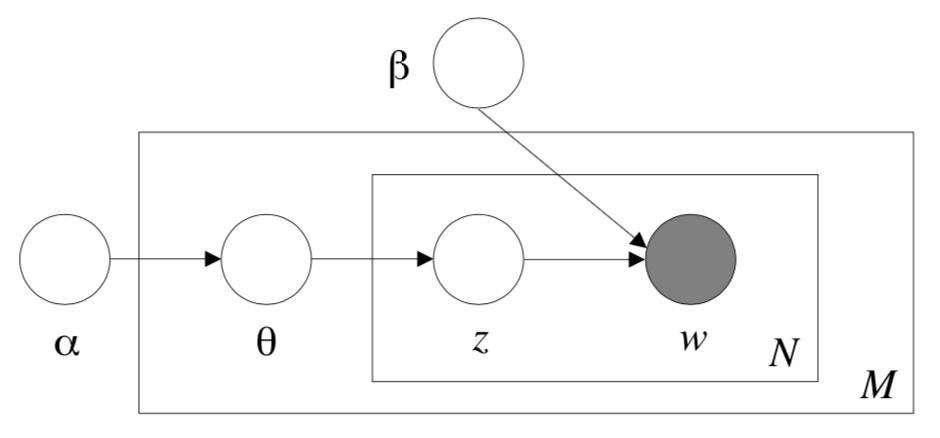
\includegraphics[scale=0.5]{LDADiagram}
% added to description; will probably update later (viv)
\caption{Graphical model representation of LDA from \cite{blei2003latent}, for
topic mixture $\theta$ (for a collection of $M$ documents); set $z$ of $N$
topics; set $w$ of $N$ words, and corpus-level parameters $\alpha$ and $\beta$.
The boxes are ``plates'' representing replicates. The outer plate represents
documents, while the inner plate represents the repeated choice of topics and
words within a document.}
\end{figure*}

Current research attempts to supplant the probabilistic modeling with a neural
network architecture.

Additional inspiration comes from Variational Auto-Encoders (VAE).

% Expand discussion on VAE and similarity to our proposal. Maybe include VAE
% diagram.

%------------------------------------------------------------------------------

\section{Original Formulation}

% Can steal shorten version from original paper! yay!
% See if we can shorten or phrase it better. This should just be a reminder of
% what we did

IBM Model 1 estimates the translation probabilities of the data through the EM
algorithm\footnote{\url{http://mt-class.org/jhu/assets/papers/alopez-model1-tutorial.pdf}}.
The EM algorithm is useful in discovering and learning the parameters of a
latent variable model. In the original IBM Model 1, this is the translation
probability distribution $t(e_i|f_j)$.

Dyer et al. \cite{dyer2013simple} added an effective reparameterization
of IBM Model 2 to produce alignment distribution $a$. We define (for a French
sentence \textbf{f} of length $n = |\textbf{f}|$, an English sentence \textbf{e}
of length $m=|\textbf{e}|$, with precision parameter $\lambda$) this alignment
distribution $a$ as follows:

\begin{equation}
\begin{split}
h(i,j,m,n) = - \left| \frac{i}{m} - \frac{j}{n}\right| \\
\\
a(i,j,m,n) =e^{  \lambda h(i,j,m,n)} \\
\end{split}
\end{equation}

This formulation gives us a positionally-aware distribution that favors alignments
towards the diagonal for a given English word $e_i$ and French word $f_j$. The
precision parameter $\lambda$ controls how strongly the model prefers the
diagonal.

Once we are done training the model, to make an alignment guess, we must find
the alignment that returns the maximum probability. For some alignment $a_i$:
\begin{equation}
\hat{a}_i = \argmax_{a_i} \, t(e_{a_i}|f_j) \cdot a(i, j, m, n)
\end{equation}
where $t(e_{a_i}|f_j)$ is the translation probability, and an alignment
distribution $a$ with parameters $\lambda$ and $p_0$. This will give us the
English word $e_{a_i}$ that is the most likely translation of the French word
$f_j$.

Finally, incorporating the Alignment by Agreement model improvement was
inspired by the work done by Liang et al. \cite{liang2006alignment}. However,
our original implementation was strongly influenced by the pseudocode used in
the \texttt{Grow-Diag-Final} Alignment Heuristic by the Moses Statistical
Translation
System\footnote{\url{http://www.statmt.org/moses/?n=FactoredTraining.AlignWords}}.

We trained an EM model in both directions, one for English-to-French,
$A_{E \rightarrow F}$, and another for French-to-English,
$A_{F \rightarrow E}$. Using the alignments generated by each individual model,
we then took the intersection of each model's alignments.

\begin{equation}
Intersection = A_{E \rightarrow F} \, \bigcap \, A_{F \rightarrow E}
\end{equation}
\begin{equation}
Union = A_{E \rightarrow F} \, \bigcup \, A_{F \rightarrow E}
\end{equation}

This effectively gave an alignment matrix that both models favored strongly
(i.e., agreed on). From this intersection matrix, we then used the
\texttt{GROW-DIAG-FINAL} algorithm to fill in the remaining gaps from the union
of alignments.

\begin{figure}
\centering
\begin{tikzpicture}

  % Define nodes
  \node[obs]                               (t) {$t$};
  \node[latent, above=0.75cm of t] (a) {$a$};
  \node[latent, above=0.75cm of a, xshift=-0.6cm] (lambda) {$\lambda$};
  \node[latent, above=0.75cm of a, xshift=0.6cm]  (null) {$p_0$};
  \node[obs, right=0.75cm of t]            (s) {$s$};
  \node[latent, below=0.95cm of t]            (theta) {$\theta$};

  % Connect the nodes
  \edge {null,lambda} {a} ; %
  \edge {a,s, theta} {t} ; %

  % Plates
  \plate [xscale=1.75, yscale=1.25] {t} {(a)(t)} {$\quad$} ;

\end{tikzpicture}
\caption{Our probabilistic plate diagram for word alignment, where $t$ is
target, $s$ is source, $\theta$ is the translation model, $\lambda$ is a
position distortion parameter, $p_0$ is the null probability, and $a$ is the
alignment distribution.}
\end{figure}

%------------------------------------------------------------------------------

% talk about NN formulation, see hand notes
\section{Neural Network Architecture}

We describe our model architecture to learn word alignments, along with
a combined loss function that will encode alignment by
agreement for both source-to-target and target-to-source embeddings.

% from a text from achintya, needs work
% While in VAEs you sample from the distribution, our model's distribution is
% discrete. Therefore we don’t have to sample and can compute in terms of all
% possibilities.


\subsection{Model Description}

Our model will consist of two parts: the pseudo E-Step prediction network, and
the pseudo M-Step evaluation (loss) function.

This prediction network accepts two inputs, a target sentence $t$ and source
sentence $s$. The network will then output an alignment matrix $\psi$, where
each rows corresponds to a source word $s_i$ and each column corresponds to a
target word $t_i$. This will help in consistency of future operations.

\begin{equation}
  \centering
\begin{array}{c|ccccc}
\psi & t_1       & \hdots & t_j       & \hdots & t_m       \\ \hline
s_1  & \psi_{11} & \hdots & \psi_{1j} & \hdots & \psi_{1m} \\
\vdots  & \vdots & \ddots & \vdots &  & \vdots \\
s_i  & \psi_{i1} & \hdots & \psi_{ij} & \hdots & \psi_{im} \\
\vdots  & \vdots &  & \vdots & \ddots & \vdots \\
s_n  & \psi_{n1} & \hdots & \psi_{nj} & \hdots & \psi_{nm}
\end{array}
\end{equation}

The prediction network mimics the E-Step by learning alignments and outputting
a $\psi$ matrix that can be thought of as a similarity matrix for every target
word $t_j$ and source word $s_i$. We define the length of the target sentence
$|t| = m$ and the length of the source sentence as $|s|=n$. Hence the $\psi$
matrix is an $n \times m$ matrix containing measures of similarity between the
$j$-th target word and $i$-th source word.

We have several ideas on how we can generate this alignment matrix $\psi$:
\begin{enumerate}
  \item Given a target word embedding $W_t$ and source word embedding $W_s$, we
    can take the element-wise dot product. So for each $t_j$, $s_i$ pairing:
  \begin{equation}
    \psi_{ij} = W_t[t_j] \cdot W_s[s_i]
  \end{equation}
  \item Use word embeddings and bi-directional LSTMs to generate alignment
    matrix $\psi$ that considers the whole sequence for both sentences.
  \item Explore deeper, more complex architectures to create a $n \times m$
    alignment matrix $\psi$.
\end{enumerate}

\begin{figure}
\centering
\begin{tikzpicture}

  % Define nodes
  \node[latent] (psi) {$\psi$};
  \node[latent, above=0.95cm of psi] (a) {$a$};
  \node[obs, above=0.85cm of a, xshift=-0.6cm] (t) {$t$};
  \node[obs, above=0.85cm of a, xshift=0.6cm] (s) {$s$};
  \node[latent, below=0.75cm of psi] (p) {$-\log p(t, s | \theta, \psi)$};
  \node[latent, left=0.75cm of p] (kl) {$D_{\mathrm{KL}} ( \sigma_t(\psi) \| a_0)$};
  \node[latent, right=0.75cm of psi] (theta) {$\theta$};
  \node[latent, below=0.95cm of p] (sum) {$\Sigma$};
  \node[latent, below=0.95cm of sum] (loss) {$Loss$};

  % Connect the nodes
  \edge {t,s} {a} ; %
  \edge {a} {psi} ; %
  \edge {psi} {kl} ; %
  \edge {psi, theta} {p} ; %
  \edge {p, kl} {sum} ; %
  \edge {sum} {loss} ; %

  % Plates
  \plate [yscale=1.25, yshift=.1cm] {t} {(a)} {} ;

\end{tikzpicture}
\caption{Model Architecture for Source $s$ to Target $t$ alignments. Neural
Network Alignment Model $a$ generates alignment matrix $\psi$. $\theta$ are
learnable translation probabilities. Evaluation function
$- \log p(t, s | \theta, \psi)$ and KL Divergence $D_{\mathrm{KL}}$ produce our
loss function to be minimized.}
\end{figure}


\subsection{Loss Functions}

To create our loss functions, we convert our alignment matrix $\psi$
to a probability distribution. Let us define $\sigma(\vec{x})$ to be
the softmax operator applied on vector $\vec{x}$, and $\sigma(\vec{x})_i$ is
the $x_i$ softmax probability for vector $\vec{x}$.

\begin{equation}
\sigma(\vec{x})_i = \frac{\exp(x_i)}{\sum_j\exp(x_j)}
\end{equation}

We therefore define two operations on the alignment matrix $\psi$. For source
$s$ to target $t$ probability generations, we define $\sigma_t(\psi)$ as the
softmax on each column, i.e. $t_j$ target word.
\begin{equation}
  \sigma_t(\psi) = \left[
    \begin{matrix}
      \sigma(\psi_{t_1}) &
      \hdots &
      \sigma(\psi_{t_j}) &
      \hdots &
      \sigma(\psi_{t_m})  \\
    \end{matrix}
\right]
\end{equation}

In addition, we further define the target-to-source generation as
$\sigma_s(\psi)$, where the softmax operator is applied on each row for target
word $s_i$ and produces a row vector.
\begin{equation}
  \sigma_s(\psi) = \left[
    \begin{matrix}
      \sigma(\psi_{s_1})  \\
      \vdots \\
      \sigma(\psi_{s_i})  \\
      \vdots \\
      \sigma(\psi_{s_n})  \\
    \end{matrix}
\right]
\end{equation}

While VAEs sample from the probability distribution derived by the neural
network, our model's distribution is discrete. Therefore, we need not
sample and can instead compute the loss in terms of all possibilities.

The following subsections describe our loss functions:

\subsubsection{Probability Maximization}

In the original formulation, we maximized probabilities for word
alignments. For this model, we define $p(t, s | \theta, \psi)$ as such:

\begin{equation}
  \begin{split}
  p(t, s | \theta, \psi)
    &= \prod_j^{|t|} \sum_i^{|s|} p_\theta(t_j| s_i) \cdot p_a(i|j) \\
    &= \prod_j^{|t|} \sum_i^{|s|} \sigma_t(\theta(t_j, s_i)) \cdot \sigma_t(\psi)_{ij}
  \end{split}
\end{equation}

This formula stems from the fact that we are assuming the alignments for each
target word $t_j$ are independent of each other, hence a product over target
words $t_j$. Then we sum over all the alignment possibilities from the source
words $s_i$, thus marginalizing over the alignments.

However, we do not maximize in neural networks, and must thus transform this
equation into a minimization problem by taking the negative logarithm of $p$.

\begin{equation}
  \begin{split}
  -\log p(t, & s | \theta, \psi) = \\
  - \sum_j^{|t|}
    & \log \left[ \sum_i^{|s|} \sigma_t \left( \theta(t_j, s_i) \right) \cdot
      \sigma_t(\psi)_{ij} \right]
\end{split}
\end{equation}

We can simplify this into the below, for easier implementation via PyTorch's
\texttt{logsumexp} function:

\begin{equation}
  \centering
  \begin{split}
  -\log  p(t & , s | \theta, \psi) = \\
  - \sum_j^{|t|} & \log \left[ \sum_i^{|s|} \exp
      \left( \log \sigma_t(\theta(t_j, s_i)) + \log \sigma_t(\psi)_{ij} \right)
    \right]
\end{split}
\end{equation}

This is the term to be minimized for the source-to-target word alignment
generation.


\subsubsection{KL Divergence and Prior Terms}

We also need to minimize the Kullback-Leibler (KL) divergence between our
distribution and a prior. For discrete probability distributions $P$ and $Q$
defined on the same probability space, the reverse KL divergence from $Q$ to
$P$ is defined as:

\begin{equation}
D_{\mathrm{KL}}(Q \| P) = \sum_{i} Q(i) \log \left( \frac{Q(i)}{P(i)} \right)
\end{equation}

In other words, it is the expectation of the logarithmic difference between the
probabilities $P$ and $Q$, where the expectation is taken using the
probabilities $Q$.

In order to calculate the KL divergence of our model, we must define
distributions $P$ and $Q$. First, we consider $P$ as our prior
distribution, henceforth called $a_0$. This prior distribution $a_0$ is a
$n \times m$ matrix filled with the alignment probabilities filled for a source
word $s_i$, target word $t_j$, source sentence $s$ of length $n$, and target
sentence $t$ of length $m$:

We define distortion exponent $h$ as:
\begin{equation}
  h(i, j) = {-\lambda \left| \frac{i}{n} - \frac{j}{m}\right|}
\end{equation}

\begin{equation}
  Z_i = \sum_{j'} \exp h(i, j')
\end{equation}

\begin{equation}
a_0 (i, j) =
\begin{cases}
      p_0 & \text{if } null \\
     (1-p_0) \cdot \frac{e^{h(i,j)}}{Z_i} & \text{else}
   \end{cases}
\end{equation}

In \cite{dyer2013simple}, parameter values were selected as $\lambda=4$ and $p_0=0.08$
for the entire corpus. Each row of $a_0$ is normalized by the sum of the row
distortion values to create a valid distribution via term $Z_i$.
We can then write our KL Divergence, which is to be minimized, as:

\begin{equation}
  D_{\mathrm{KL}}(\sigma_t(\psi) \| a_0) =
    \sum_i^n \sum_j^m \sigma_t(\psi)_{ij} \cdot
      \log \left[ \frac{\sigma_t(\psi)_{ij}}{a_0(i, j)} \right]
\end{equation}


\subsubsection{Target-to-Source Loss Terms}

We have described the loss terms for a source $s$ to target $t$ word alignment.
However, we seek to perform alignment by agreement. Hence we need to add loss
functions that describe the evaluation of target $t$ to source $s$. Hence, we
add terms:

\begin{equation}
  \centering
  \begin{split}
  -\log  p(t & , s | \theta, \psi) = \\
  - \sum_i^{|s|} & \log \left[ \sum_j^{|t|}
      \exp \left(
        \log \sigma_s(\theta(t_j, s_i)) + \log \sigma_s(\psi)_{ij}
      \right)
    \right]
\end{split}
\end{equation}

And now for the KL Divergence term for target $t$ to source $s$:

\begin{equation}
D_{\mathrm{KL}} (\sigma_s(\psi) \| a_0) = \sum_i^n \sum_j^m \sigma_s(\psi)_{ij}
  \cdot \log \left[ \frac{\sigma_s(\psi)_{ij}}{a_0(i, j)} \right]
\end{equation}

Where the normalization of the prior $a_0$ is on the column instead of the row.
We also perform the softmax operator on each column of the $\psi$ matrix,
previously defined as $\sigma_t(\psi)$


\subsubsection{Alignment by Agreement}

Finally, one last loss function term must be added to jointly train each model.
We define $\circ$ as the Hadamard Product, which is the element wise
multiplication of two matrices. For instance:
$(A \circ B)_{ij} = A_{ij} \cdot B_{ij}$. We can write the term as such:

\begin{equation}
  -\log \sum_i^{|s|} \sum_j^{|t|}
    \left[ \sigma_s(\psi) \circ \sigma_t(\psi) \right]_{ij}
\end{equation}

% Again note here, you can use logsumexp trick to implement this efficiently in
% PyTorch


\subsubsection{Combined Loss Function}

Our final loss function, to be minimized, is a 5-term equation. We define $a_t$
as the prior alignment matrix $a_0$ normalized per column, $a_s$ as the prior
alignment matrix normalized per row, $\sigma_s$ as the softmax operator applied
on the rows of a matrix, and $\sigma_t$ as the softmax operator applied to each
column of a matrix. Indexing is done under the assumption that source words
$s_i$ form rows, and target words $t_j$ form columns, and $ij$ is a shorthand
for $s_i$ and $t_j$ indexing into our matrices.

\begin{equation}
  \centering
\begin{split}
  Lo&ss = \\
  &- \sum_j^{|t|} \log \left[
      \sum_i^{|s|} \exp \left(
        \log \sigma_t(\theta(t, s))_{ij} + \log \sigma_t(\psi)_{ij} \right)
    \right] \\
  &+ \sum_i^n \sum_j^m \sigma_t(\psi)_{ij} \cdot \log \left[
    \frac{\sigma_t(\psi)_{ij}}{a_t(i, j)} \right] \\
  &- \sum_i^{|s|} \log \left[ \sum_j^{|t|}
      \exp \left(
        \log \sigma_s(\theta(t, s))_{ij} + \log \sigma_s(\psi)_{ij}
      \right)
    \right] \\
  &+ \sum_i^n \sum_j^m \sigma_s(\psi)_{ij} \cdot \log \left[
    \frac{\sigma_s(\psi)_{ij}}{a_s(i, j)} \right] \\
  &- \log \sum_i^{|s|} \sum_j^{|t|} \left[
    \sigma_s(\psi) \circ \sigma_t(\psi) \right]_{ij} \\
\end{split}
\end{equation}

% Note, the alignment prior is not exactly the same for source-to-target and
% target-to-source because even though the loss function is symmetric, the
% probabilities are normalized with respect to n or m, depending which
% direction you are translating


\subsection{Prediction}

For prediction, we can set a threshold for our alignment matrix $\psi$ and take
it as our alignments.

%------------------------------------------------------------------------------

\section{Data}

% talk about subtitle extraction. Also labeling of data for supervised? Or
% should that go in supervised training section. Get Bailey to mention Nikita
% metric for baseline on unaligned corpus.


\subsection{Introduction}

The efficacy of a neural network alignment system depends heavily on the
quality and quantity of the training data available. We look to leverage
existing corpora of natural language in various settings instead of the
traditional corpora (such as the Europal, which are domain specific and lack
the unstructured and informal nature of typical language use). Training on
these commonly used corpora leads to models with preferences for emitting
language of a parliamentary nature, for example. We elect to focus on corpora
that provide more of a contextual breadth.

To this end, amassed a corpus of domestic and international movie and TV show
subtitles from a variety of sources. Subtitles have the unique advantage of
being already sentence-aligned thanks to timestamps. Additionally, this
alignment somewhat holds even if timestamps are skewed between different media
formats of the same source with slightly different timings. We plan to handle
subtitles in strict alignment (that is, those whose timestamps exactly
correspond) and also will attempt to sentence-align those that are in fuzzy
alignment (timestamps do not correspond one-to-one). For more on our
methodology, see \hyperref[subsec:subtitle-alignment]{Subtitle Alignment}.

Our preference was to collect only professional or official subtitles, but
unfortunately these fall under copyright law and are often not publicly
available. However, there are communities of volunteer transcribers and
translators from which we can obtain unofficial subtitles. Many of these
communities have databases with publicly available dumps of all translations,
offer an API, or have a website that is scrapeable. We have employed these
tactics to obtain an initial corpus (see
\hyperref[subsec:procuring-subtitles]{Procuring Subtitles}).

For evaluating the effectiveness of our model and to facilitate
\hyperref[sec:supervised-training]{Supervised Training} we need ground truth
alignments of some subset of our corpus. As we later discuss, or corpus
currently has 90 million English-French aligned subtitles (each approximately
consisting of one sentence). This is, of course, impractical to align by hand
even with significant resources. So, we are presented with a similar evaluation
problem that that in Liu et al. \cite{liu2015streaming}. However, instead of
the ground truth being intractable, our ground truth is impractical to compute.
We elect to obtain ground truth alignments by a similar consensus based
approach to that in \cite{liu2015streaming}. Broadly, we look to well-known
open-source alignment software en masse to provide an approximation of the
ground truth alignments. We do so by evaluating the pairwise overlap between
each aligner and our model to determine a metric that can approximate
Alignment Error Rate (AER) (see
\hyperref[subsec:ground-truth-alignments]{Ground Truth Alignments}).


\subsection{Procuring Subtitles}
\label{subsec:procuring-subtitles}

% TODO


\subsection{Subtitle Alignment}
\label{subsec:subtitle-alignment}

% TODO


\subsection{Ground Truth Alignments}
\label{subsec:ground-truth-alignments}

% TODO

%------------------------------------------------------------------------------

\section{Training}

% discuss implementation ideas and why we feel like this will work.


\subsection{Supervised Training}
\label{sec:supervised-training}

% Cut out top part of model, talk about how we will label our data and
% incorporate


\subsection{Unsupervised Training}

% 5 term loss function
% most likely will be:
% priors are sim to KL div
% = prior f to e + prior e to f + logprob f to e + logprob e to f + alignment
%     by agreement

%------------------------------------------------------------------------------

\section{Expectation}

% Our Hopes and Dreams!

%------------------------------------------------------------------------------

% References
\bibliographystyle{abbrv}
\bibliography{project_proposal}

\end{document}
